% !TEX root = ../../main.tex
\section{Genetic drift and the stochastic nature of evolution}

So far we have studied two of the forces of evolution from a deterministic
perspective. This sounds contradictory given the intuition that biologists have
about how the evolutionary process works. On the one hand any biologist will
tell you that evolution is a completely random process; from the emergence of a
beneficial mutation to the process of fixing this mutation in the population,
these dynamics are hard if not impossible to predict.

On the other hand in a conflicting view of evolution, biologists tend to
associate every biological feature to a product of selection. Either by natural
or sexual selection, the literature is full of ``just-so-stories'' that
attribute a functional purpose to every aspect of biological systems. Therefore
the claim is that the process occurs at random, but everything serves a
purpose. The truth most likely lies somewhere in between.

At the dawn of the modern synthesis of evolutionary theory Sewall Wright came
to the conclusion that reproductive stochasticity could play an important role
in the fate of populations. In other words, not because a beneficial mutation
appeared in the population it would necessarily take over the population; or
not because a deleterious mutation appeared in the population it would be
immediately removed. Accidents in evolution still play an important role when
it comes to setting the fate of a population. From a beneficial mutation being
lost due to some non-selection related event such as a stochastic death of the
organism carrying the mutation, to the fixation of deleterious mutations in the
population. The first experimental demonstration of this non-selection based
evolution came out of Wrights own academic lineage. His own student, Peter
Buri, designed the first experiment to demonstrate the force of genetic drift.

\subsection{The Buri experiment}

\mrm{This section will probably live in the discrete evolution part of the 
notes once they exist. But for now I want to use Buri to motivate the reason
for thinking about drift. It doesn't necessarily fit with the bacteria-centered
tone of the notes, but it is such a great experiment!}

In 1956 Peter Buri, a student of Sewall Wright published the now classic paper
``\textit{Gene Frequency in Small Populations of Mutant Drosophila}'' in which
he experimentally demonstrated the concept of genetic drift.  The idea for this
beautiful experiment is depicted in \fref{fig_02_buri_schematic}. Briefly, Buri
began with eight female and eight male flies, all heterozygotes of the
\textit{bw} locus. This means that all of the flies had 1 copy of the gene
associated with white eyes, and one copy of the gene associated with  red eyes.
The phenotype that this combination of alleles gives is flies with orange eyes.
He then allowed the flies to reproduce, and after removing the adults, he
randomly chose 8 males and females from the next generation of offspring
without looking at the eye color. These new 8 males and 8 females were
transferred to a new flask and the procedure was repeated for 19 generations.

\begin{figure}[h!]
\centering 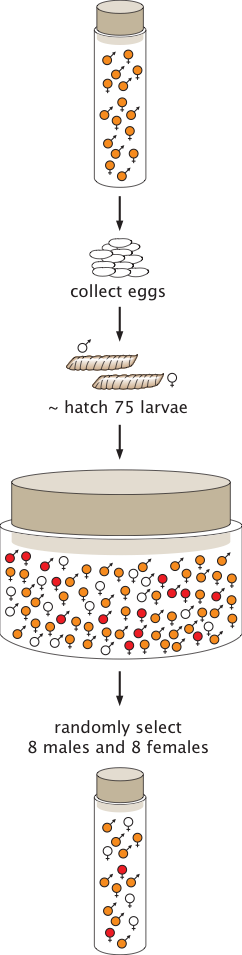
\includegraphics[scale=0.8]
  {../fig/drift_langevin/02_01_01_buri_schematic.png}
  \caption{\textbf{Buri's experimental setup.} At time $t=0$ eight
  heterozygote females and eight heterozygote males were allowed to reproduce.
  From their offspring, eight males and eight females were chosen at random and
  transferred into a new flask.}
  \label{fig_02_01_01}
\end{figure}

Since the offspring that made it to the next generation were chosen at random,
Buri knew that the outcome would be different if he repeated an identical
experiment in different vials. As a result, for statistical power he
simultaneously tracked 107 flasks as shown in \fref{fig_02_01_01}.
Each generation, he counted the number of red-eyed, white-eyed and orange-eyed
flies he had randomly chosen. \fref{fig_02_01_02} shows the outcomes
for these different vials after 19 generations. Because the flies are allegedly
mating at random, with each generation there is an accumulation of
fluctuations. As a result, after 19 generations, many vials contained only
white-eyed or red-eyed flies, though some vials still contained a mixture of
eye colors.

\begin{figure}[h!]
\centering 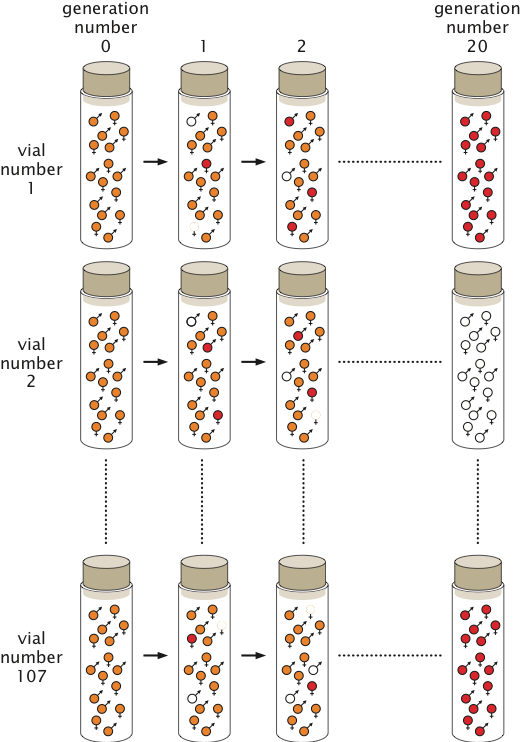
\includegraphics[scale=0.7]
  {../fig/drift_langevin/02_01_02_buri_generations.png}
  \caption{\textbf{Multiple replicates of the Buri experiment.}  Buri repeated
  his experiment in 107 separate vials, with the evolutionary trajectory
  different each time as a result of genetic drift.  Note that in the long time
  limit, many of the vials have gone to fixation with all flies having either
  white or red eyes.}
\label{fig_02_01_02}
\end{figure}

Having quantified the number of red-eyed, white-eyed and orange-eyed flies Buri
was able to quantify the frequency of alleles in the population. Since none of
the alleles were dominant, he could infer the genotype  by looking at the
phenotype of the flies.

\fref{fig_02_01_03} summarizes the results of the experiment. By
tracking alleles over time with these 107 populations exposed to the same
conditions, Buri was able to observe evolution driven entirely by genetic
drift! He saw how in some of the populations one of the alleles went extinct,
arising from nothing more than the fluctuations inherent in small populations.

\begin{figure}[h!]
\centering
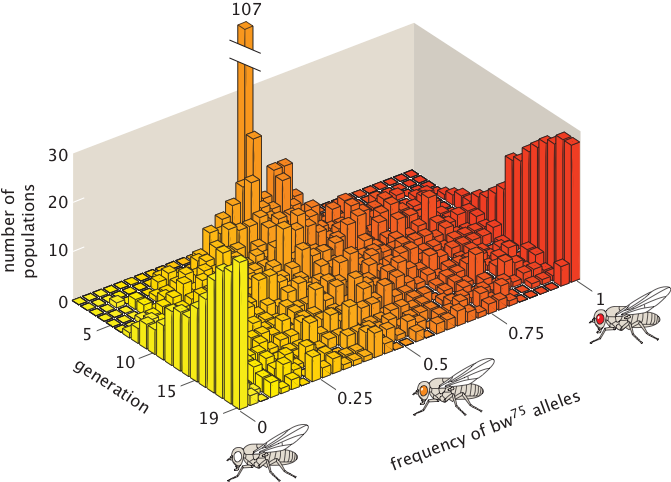
\includegraphics[scale=0.85]
  {../fig/drift_langevin/02_01_03_buri_experiment.png}
  \caption{\textbf{Results of the Buri experiment.} By tracking the phenotypes
  of the  flies, Buri was able to infer the allele frequencies for each
  population. The allele frequencies change as a result of genetic drift and
  after 19 generations, many of the vials contain flies all with the same eye
  color, implying fixation of alleles and evolution due to genetic drift.}
  \label{fig_02_01_03}
\end{figure}

Now that we have looked at an experimental evidence of genetic drift on a
laboratory experiment let's go back to the mathematical modeling of this
phenomena.